%=============================================================================
% SECTION 12: COSMOLOGICAL IMPLICATIONS
% Part VII: Cosmology and Open Problems
% v2.9+: ψ-Tomography (ψ-Screen) inverse-first cosmology module
%=============================================================================

\section{Cosmological Implications}\label{sec:cosmology}

DFD cosmology is treated as an \emph{inverse optical problem}: infer the line-of-sight optical bias field directly from data, and only then interpret what standard cosmology would call ``expansion history,'' ``dark energy,'' and ``dark matter.'' In this framing, GR/$\Lambda$CDM enters \emph{only} as an observer dictionary (how distances/angles are commonly reported), not as ontology.

%=============================================================================
% ψ-TOMOGRAPHY (ψ-SCREEN) COSMOLOGY MODULE
%=============================================================================
\subsection{$\psi$-Tomography ($\psi$-Screen) Cosmology Module}\label{sec:psi-tomography}

\paragraph{Non-negotiable premise.}
The primary reconstructed object is the ``$\psi$-screen'' on the past light cone:
\begin{equation}
\Delta\psi(z,\hat n)\;\equiv\;\psi_{\rm em}(z,\hat n)\;-\;\psi_{\rm obs},
\qquad \text{dimensionless.}
\label{eq:psitomo-def-dpsi}
\end{equation}
All GR/$\Lambda$CDM quantities used in this section (e.g.\ $D_L^{\rm dict},D_A^{\rm obs}$) are \emph{reporting-layer} variables that serve as a convenient dictionary for published datasets.

%-----------------------------------------------------------------------------
\subsubsection{DFD postulates and sign conventions}

DFD is formulated on flat $\mathbb{R}^3$ with a scalar field $\psi$ and refractive index $n=e^\psi$.
The one-way light speed is
\begin{equation}
c_1(\psi)=c\,e^{-\psi},
\end{equation}
and the (nonrelativistic) acceleration of matter is
\begin{equation}
\bm a \;=\;\frac{c^2}{2}\,\nabla\psi.
\label{eq:psitomo-accel}
\end{equation}
We adopt the gauge choice $\psi_{\rm obs}\equiv 0$, so that $\Delta\psi=\psi_{\rm em}$ in this gauge. With this convention:
\begin{itemize}
\item $\Delta\psi>0$ means $\psi$ (hence $n$) was higher at emission than locally (slower $c_1$ at emission).
\item $\Delta\psi<0$ means $\psi$ was lower at emission than locally (faster $c_1$ at emission).
\end{itemize}

\paragraph{Endpoint vs.\ observable screen.}
Equation~\eqref{eq:psitomo-def-dpsi} is an endpoint definition.
Operationally, each dataset reconstructs an \emph{observable} screen $\Delta\psi_{\rm obs}$ defined by the log-multiplicative bias required by the DFD optical relations below.
When needed, one may represent $\Delta\psi_{\rm obs}$ as a weighted line-of-sight functional
\begin{equation}
\Delta\psi_{\rm obs}(z,\hat n)
=\int_{0}^{\chi(z)}\!d\chi\;W_{\rm obs}(\chi;z)\,\delta\psi(\chi,\hat n),
\label{eq:psitomo-los-functional}
\end{equation}
where $\chi$ is a dictionary comoving-distance coordinate and $W_{\rm obs}$ is a dataset-specific kernel.
The inverse program reconstructs $\Delta\psi_{\rm obs}$ \emph{directly from data} without assuming a particular $W_{\rm obs}$.

%-----------------------------------------------------------------------------
\subsubsection{Forward model: three primary DFD optical relations}

The module is built around three primary DFD optical relations.

\paragraph{(1) Luminosity-distance bias (SNe Ia).}
Let $D_L^{\rm dict}(z,\hat n)$ be the baseline luminosity distance as typically reported under the observer dictionary.
DFD maps this to an optically biased luminosity distance:
\begin{equation}
D_L^{\rm DFD}(z,\hat n)=D_L^{\rm dict}(z,\hat n)\,e^{\Delta\psi(z,\hat n)}.
\label{eq:psitomo-DL-bias}
\end{equation}
Equivalently, $\ln D_L^{\rm DFD}=\ln D_L^{\rm dict}+\Delta\psi$.

\paragraph{(1b) Angular-diameter-distance bias.}
Both $D_L$ and $D_A$ are computed from null geodesics of the same optical metric $\tilde g_{\mu\nu}$. The $\psi$-field therefore screens both distances equally:
\begin{equation}
D_A^{\rm DFD}(z,\hat n)=D_A^{\rm dict}(z,\hat n)\,e^{\Delta\psi(z,\hat n)}.
\label{eq:psitomo-DA-bias}
\end{equation}

\paragraph{(2) Distance duality (Etherington reciprocity).}\label{sec:psitomo-duality}
DFD's optical metric $d\tilde s^2 = -c^2\,dt^2/n^2 + d\mathbf{x}^2$ with $n = e^\psi > 0$ is a smooth, non-degenerate Lorentzian metric. All three conditions of Etherington's reciprocity theorem\cite{Etherington1933,Ellis2007} are satisfied: (i)~photons propagate on null geodesics of a Lorentzian metric; (ii)~geodesics are locally unique ($\psi$ is $C^{1,\alpha}$ away from sources, Appendix~\ref{app:wellposedness}); (iii)~photon number is conserved (no absorption/emission mechanism). Therefore
\begin{equation}
D_L(z,\hat n) \;=\; (1+z)^2\,D_A(z,\hat n).
\label{eq:psitomo-duality}
\end{equation}
This holds exactly; no $e^{\Delta\psi}$ factor appears. The common screening factor from Eqs.~\eqref{eq:psitomo-DL-bias} and \eqref{eq:psitomo-DA-bias} cancels in the ratio $D_L/D_A$.

\paragraph{Notation.} We distinguish $\Delta\psi_{\rm screen}(z,\hat n)$ (the distance bias relative to the dictionary baseline, measured by Estimators~A and~C below; can be large, $\approx 0.27$ at $z=1$) from $\Delta\psi_{\rm dual}(z,\hat n) \equiv \ln[D_L/(1+z)^2 D_A] = 0$ (the DDR violation parameter, measured by Estimator~B; identically zero). Where the subscript is omitted, $\Delta\psi$ refers to $\Delta\psi_{\rm screen}$.

\paragraph{(3) CMB acoustic-scale screen (angular anisotropy).}
Let $\ell_1(\hat n)$ denote the locally inferred first acoustic peak location from patchwise CMB power spectra.
DFD posits the angular screen mapping
\begin{equation}
\ell_1(\hat n)=\ell_{\rm true}\,e^{-\Delta\psi(\hat n)},
\label{eq:psitomo-cmb-ell1}
\end{equation}
where $\ell_{\rm true}$ is a sky-independent constant that cancels out of the normalized anisotropy reconstruction below.

\paragraph{Sign of the $\ell_1$ mapping.}
The sign deserves explicit comment.  The distance relations Eqs.~\eqref{eq:psitomo-DL-bias}--\eqref{eq:psitomo-DA-bias} give $D_A^{\rm DFD} \propto e^{+\Delta\psi}$: objects appear \emph{farther}, which naively pushes $\ell_1 \propto D_A/r_s$ \emph{higher}.  But that scaling applies to the sky-averaged monopole, which is absorbed into $\ell_{\rm true}$.  Equation~\eqref{eq:psitomo-cmb-ell1} describes the \emph{direction-dependent} anisotropy: a foreground sightline with $\Delta\psi(\hat n) > 0$ acts as a convergent screen that \emph{magnifies} the angular scale of CMB features in that patch.  Larger apparent angular scale maps to \emph{lower} $\ell_1$, hence the negative exponent.  This is the same sign as standard weak-lensing magnification of the CMB, where convergence $\kappa > 0$ shifts power to lower $\ell$.

%-----------------------------------------------------------------------------
\subsubsection{Two independent screen estimators and one consistency check}\label{sec:psitomo-estimators}

\paragraph{Estimator A: SNe Ia alone (and its degeneracy).}
From Eq.~\eqref{eq:psitomo-DL-bias}, an operational estimator on each SN sightline is
\begin{equation}
\widehat{\Delta\psi}_{\rm SN}(z_i,\hat n_i)
\;\equiv\;
\ln D_L^{\rm obs}(z_i,\hat n_i) - \ln D_L^{\rm dict}(z_i) - \mathcal{M},
\label{eq:psitomo-est-sn}
\end{equation}
where $\mathcal{M}$ is an unknown constant absorbing absolute magnitude / distance-ladder calibration.
SNe alone cannot fix an additive constant in $\Delta\psi$ (monopole), because $\Delta\psi\!\to\!\Delta\psi+{\rm const}$ can be absorbed into $\mathcal{M}$.
A robust SN-only product is therefore the anisotropy field
\begin{equation}
\widehat{\delta\psi}_{\rm SN}(z,\hat n)\;\equiv\;\widehat{\Delta\psi}_{\rm SN}(z,\hat n)-\big\langle \widehat{\Delta\psi}_{\rm SN}(z,\hat n)\big\rangle_{\hat n}.
\label{eq:psitomo-est-sn-aniso}
\end{equation}

\paragraph{Estimator B: SNe + BAO / strong lensing (duality consistency check).}
Etherington's reciprocity~\eqref{eq:psitomo-duality} implies that the observable ratio
\begin{equation}
\boxed{
\widehat{\Delta\psi}_{\rm dual}(z,\hat n)
\;\equiv\;\ln\!\left(\frac{D_L^{\rm obs}(z,\hat n)}{(1+z)^2\,D_A^{\rm obs}(z,\hat n)}\right)
\;=\; 0.
}
\label{eq:psitomo-est-dual}
\end{equation}
This is not an independent measurement of $\Delta\psi_{\rm screen}$; it is a \emph{consistency check} that the optical metric satisfies Etherington's conditions. Observational confirmation ($\widehat{\Delta\psi}_{\rm dual} = 0.01 \pm 0.02$)\cite{Holanda2010,Liang2011} validates the metric structure.

\paragraph{Estimator C: CMB peak anisotropy (screen at last scattering).}
From Eq.~\eqref{eq:psitomo-cmb-ell1}, define the normalized estimator:
\begin{equation}
\boxed{
\widehat{\Delta\psi}_{\rm CMB}(\hat n)
= -\ln\!\left(\frac{\ell_1(\hat n)}{\langle\ell_1\rangle}\right),
}
\label{eq:psitomo-est-cmb}
\end{equation}
which fixes the additive constant by construction ($\langle\widehat{\Delta\psi}_{\rm CMB}\rangle=0$). This isolates \emph{angular} structure in the screen at last scattering.

\paragraph{How to obtain $\ell_1(\hat n)$ without $\Lambda$CDM priors.}
Choose a sky patching scheme; estimate local pseudo-$C_\ell$ spectra per patch (beam/mask corrected);
fit a \emph{local peak locator} template around the first peak (only a smooth peaked function is required);
take the maximizing multipole as $\ell_1$ for that patch.

%-----------------------------------------------------------------------------
\subsubsection{Theorem-level internal closure of the reconstructed screen}
\label{sec:psitomo-closure-theorems}

The two screen estimators and one consistency check introduced above are not merely ``three ways of plotting the same thing'':
under the forward optical relations, they imply \emph{overdetermined closure identities} that must hold
on the sky (and across redshift bins) if a single scalar screen $\Delta\psi(z,\hat n)$ is the correct
organizing variable.

\paragraph{Conventions and hypotheses.}
Fix a redshift bin $z\in[z_a,z_b]$ and an analysis mask $W(\hat n)$ (common to all maps in a given test).
Assume:
\begin{enumerate}
\item \textbf{(H1) Forward relations.} The DFD optical relations~\eqref{eq:psitomo-DL-bias}--\eqref{eq:psitomo-cmb-ell1} hold on their respective domains of validity.
\item \textbf{(H2) Observable identification.} The reported distances used in Eqs.~\eqref{eq:psitomo-est-sn}--\eqref{eq:psitomo-est-dual} are the observational reconstructions of the corresponding DFD distances along that line of sight, i.e.\ $D_L^{\rm obs}(z,\hat n)=D_L^{\rm DFD}(z,\hat n)$ and $D_A^{\rm obs}(z,\hat n)=D_A^{\rm DFD}(z,\hat n)$ (up to the stated measurement errors).
\item \textbf{(H3) SN calibration constancy.} The SN absolute calibration constant $\mathcal{M}$ in Eq.~\eqref{eq:psitomo-est-sn} is a global constant (independent of $z$ and $\hat n$), as assumed in the estimator definition.
\end{enumerate}
No dynamical assumption about $\mu(x)$, growth, or a specific dictionary is required for the identities below.

\begin{theorem}[Duality consistency]\label{thm:duality-inversion}
Under (H1)--(H2), the duality estimator~\eqref{eq:psitomo-est-dual} tests Etherington consistency:
\begin{equation}
\widehat{\Delta\psi}_{\rm dual}(z,\hat n)=0.
\label{eq:closure-dual-exact}
\end{equation}
\end{theorem}

\begin{proof}
From Eqs.~\eqref{eq:psitomo-DL-bias} and \eqref{eq:psitomo-DA-bias}, both distances carry the common screening factor $e^{\Delta\psi}$. In the ratio $D_L/[(1+z)^2 D_A]$ this factor cancels, leaving the standard Etherington relation~\eqref{eq:psitomo-duality}: $D_L^{\rm dict}/[(1+z)^2 D_A^{\rm dict}]=1$. Hence $\widehat{\Delta\psi}_{\rm dual}=\ln 1=0$.
\end{proof}

\begin{theorem}[SN inversion up to an additive constant]\label{thm:sn-inversion}
Under (H1)--(H3), the SN estimator~\eqref{eq:psitomo-est-sn} satisfies
\begin{equation}
\widehat{\Delta\psi}_{\rm SN}(z,\hat n)=\Delta\psi(z,\hat n)-\mathcal{M},
\label{eq:closure-sn-offset}
\end{equation}
and therefore its centered field~\eqref{eq:psitomo-est-sn-aniso} equals the true screen anisotropy at that redshift:
\begin{equation}
\widehat{\delta\psi}_{\rm SN}(z,\hat n)=\Delta\psi(z,\hat n)-\langle \Delta\psi(z,\hat n)\rangle_{\hat n}.
\label{eq:closure-sn-aniso}
\end{equation}
\end{theorem}

\begin{proof}
From Eq.~\eqref{eq:psitomo-DL-bias}, $\ln D_L^{\rm DFD}=\ln D_L^{\rm dict}+\Delta\psi$. Using (H2) and inserting into~\eqref{eq:psitomo-est-sn} gives $\widehat{\Delta\psi}_{\rm SN}=\Delta\psi-\mathcal{M}$. Centering over $\hat n$ cancels $\mathcal{M}$ identically, yielding~\eqref{eq:psitomo-est-sn-aniso} as the true anisotropy.
\end{proof}

\begin{corollary}[A--B closure simplification]\label{cor:ab-closure}
Under (H1)--(H3), since $\widehat{\Delta\psi}_{\rm dual}=0$ (Theorem~\ref{thm:duality-inversion}) and $\widehat{\Delta\psi}_{\rm SN}=\Delta\psi_{\rm screen}-\mathcal{M}$ (Theorem~\ref{thm:sn-inversion}), the calibration constant is directly extractable:
\begin{equation}
\widehat{\mathcal{M}}(z)=
-\Big\langle \widehat{\Delta\psi}_{\rm SN}(z,\hat n)\Big\rangle_{\hat n,W}.
\label{eq:closure-ab-offset}
\end{equation}
Equivalently, defining the \textbf{internal closure residual field}
\begin{equation}
R_{AB}\equiv
\widehat{\Delta\psi}_{\rm SN}+\widehat{\mathcal{M}}
= \Delta\psi_{\rm screen} - \langle\Delta\psi_{\rm screen}\rangle_{\hat n},
\label{eq:closure-residual}
\end{equation}
recovers the screen anisotropy (up to measurement noise).
\end{corollary}

\begin{proof}
Set $\widehat{\Delta\psi}_{\rm dual}=0$ in the original A--B difference; the result follows from Theorem~\ref{thm:sn-inversion}.
\end{proof}

\begin{corollary}[Cross-bin overdetermination: $\mathcal{M}$ must be constant]\label{cor:m-constancy}
Under (H3), the offset $\widehat{\mathcal{M}}(z)$ extracted from Corollary~\ref{cor:ab-closure} is independent of redshift. In practice, for redshift bins $\{z_j\}$ with overlaps, the statistic
\begin{equation}
\chi^2_{\mathcal{M}}=\sum_j \frac{\big(\widehat{\mathcal{M}}(z_j)-\overline{\mathcal{M}}\big)^2}{\sigma_{\mathcal{M}}^2(z_j)},
\qquad
\overline{\mathcal{M}}\equiv \frac{\sum_j \widehat{\mathcal{M}}(z_j)/\sigma_{\mathcal{M}}^2(z_j)}{\sum_j 1/\sigma_{\mathcal{M}}^2(z_j)}
\label{eq:closure-chi2-m}
\end{equation}
is an \textbf{overdetermined} consistency test of the SN calibration: large $\chi^2_{\mathcal{M}}$ falsifies at least one of (H1)--(H3) (or flags unmodeled systematics).
\end{corollary}

\begin{corollary}[Harmonic-space closure for anisotropy: SN vs CMB]\label{cor:harmonic-closure}
Since $\widehat{\Delta\psi}_{\rm dual}=0$, the non-trivial harmonic closure test compares the two independent screen estimators.
Let both the centered SN map (Theorem~\ref{thm:sn-inversion}) and the CMB map (Theorem~\ref{thm:cmb-centered}) be defined on a common mask. Then for all multipoles $\ell\ge 1$:
\begin{equation}
a_{\ell m}^{\rm SN}(z_\ast)=a_{\ell m}^{\rm CMB},
\label{eq:closure-alm}
\end{equation}
where $z_\ast$ is the last-scattering redshift, and therefore (after identical smoothing/masking) the pseudo-$C_\ell$ spectra satisfy
\begin{equation}
\widehat C_\ell^{\rm SN\times SN}(z_\ast)=\widehat C_\ell^{\rm CMB\times CMB}=
\widehat C_\ell^{\rm SN\times CMB}
\qquad (\ell\ge 1),
\label{eq:closure-cl}
\end{equation}
up to the usual mask-coupling and noise-bias corrections.
\end{corollary}

\begin{proof}
Both the SN-centered map and the CMB map reconstruct the same monopole-free screen $\Delta\psi_{\rm screen}(z_\ast,\hat n)-\langle\Delta\psi_{\rm screen}\rangle_{\hat n}$ at last scattering (up to measurement noise), hence equal harmonic coefficients for $\ell\ge 1$.
\end{proof}

\begin{theorem}[CMB estimator is the centered last-scattering screen]\label{thm:cmb-centered}
Under (H1)--(H2), the CMB peak estimator~\eqref{eq:psitomo-est-cmb} reconstructs the monopole-free screen at last scattering:
\begin{equation}
\widehat{\Delta\psi}_{\rm CMB}(\hat n)=\Delta\psi(z_\ast,\hat n)-\langle\Delta\psi(z_\ast,\hat n)\rangle_{\hat n}.
\label{eq:closure-cmb}
\end{equation}
\end{theorem}

\begin{proof}
From Eq.~\eqref{eq:psitomo-cmb-ell1}, $\ell_1(\hat n)=\ell_{\rm true}e^{-\Delta\psi(\hat n)}$.
Taking $-\ln(\ell_1/\langle\ell_1\rangle)$ cancels $\ell_{\rm true}$ and removes the monopole by construction, yielding Eq.~\eqref{eq:psitomo-est-cmb}.
\end{proof}

\paragraph{Interpretation.}
Theorems~\ref{thm:duality-inversion}--\ref{thm:cmb-centered} promote ``closure'' from prose to algebra:
\emph{a single screen} $\Delta\psi_{\rm screen}(z,\hat n)$ implies (i) Etherington consistency ($\widehat{\Delta\psi}_{\rm dual}=0$), (ii) an SN reconstruction with only one global degeneracy $\mathcal{M}$, and (iii) strict agreement of SN and CMB anisotropy maps on overlapping skies and bins.
This makes $\Delta\psi_{\rm screen}(z,\hat n)$ an \emph{overconstrained} observable: independent reconstructions must agree, and persistent mismatch falsifies the single-screen hypothesis.

%-----------------------------------------------------------------------------
\subsubsection{Killer falsifier (GR-independent)}\label{sec:psitomo-falsifier}

\paragraph{Primary falsifier: cross-correlation with independent structure maps.}
Let $X(\hat n)$ be an independent line-of-sight structure tracer map (e.g.\ CMB lensing convergence $\kappa$ or a projected galaxy density map in a defined redshift slice).
Compute the cross-power spectrum
\begin{equation}
\widehat C_\ell^{\Delta\psi\times X}
\;\equiv\;
\frac{1}{2\ell+1}\sum_{m=-\ell}^{\ell}\Delta\psi_{\ell m}\,X_{\ell m}^\ast,
\label{eq:psitomo-cl-cross}
\end{equation}
and the dimensionless correlation coefficient
\begin{equation}
\widehat r_\ell
\;\equiv\;
\frac{\widehat C_\ell^{\Delta\psi\times X}}
{\sqrt{\widehat C_\ell^{\Delta\psi\times\Delta\psi}\;\widehat C_\ell^{X\times X}}}.
\label{eq:psitomo-r-ell}
\end{equation}

\paragraph{Null hypothesis (falsifier).}
\begin{equation}
H_0:\quad C_\ell^{\Delta\psi\times X}=0\quad \text{for all analyzed $\ell$ (or all bins).}
\label{eq:psitomo-null}
\end{equation}
Pre-registered falsification criterion:
\begin{quote}
\emph{If $\widehat{\Delta\psi}_{\rm CMB}(\hat n)$ (or $\widehat{\delta\psi}_{\rm SN}$ at low $z$) exhibits no statistically significant cross-correlation with an independent structure map $X(\hat n)$ down to the sensitivity implied by the measured $\Delta\psi$ auto-power and the map noises, then the $\psi$-screen mechanism (as the explanation for the optical biases in this module) is falsified.}
\end{quote}

A standard variance model for planning is
\begin{equation}
\resizebox{\columnwidth}{!}{$
\mathrm{Var}\!\left(\widehat C_\ell^{\Delta\psi\times X}\right)
\simeq \frac{1}{(2\ell+1)f_{\rm sky}}
\Big[
\left(C_\ell^{\Delta\psi\times X}\right)^2
+\left(C_\ell^{\Delta\psi\Delta\psi}+N_\ell^{\Delta\psi}\right)
\left(C_\ell^{XX}+N_\ell^{X}\right)
\Big]
$}
\label{eq:psitomo-cl-var}
\end{equation}
with sky fraction $f_{\rm sky}$ and noise power spectra $N_\ell^{\Delta\psi}$ and $N_\ell^{X}$.

\paragraph{Secondary falsifier: internal closure among estimators.}
The closure identities proved in Sec.~\ref{sec:psitomo-closure-theorems} (Theorems~\ref{thm:duality-inversion}--\ref{thm:cmb-centered} and Corollaries~\ref{cor:ab-closure}--\ref{cor:harmonic-closure}) provide quantitative falsification tests:
\begin{itemize}
\item Estimator~B must return $\widehat{\Delta\psi}_{\rm dual}=0$ (Etherington consistency)
\item The SN calibration offset $\widehat{\mathcal{M}}(z)$ must be independent of redshift
\item The centered SN and CMB anisotropy maps must agree for $\ell \ge 1$ at the last-scattering redshift
\end{itemize}
Persistent, statistically significant violation of any closure identity falsifies the ``single-screen'' hypothesis.

A separate dedicated closure-test writeup now exists in the broader DFD program, centered on pre-registered internal-closure statistics and randomized null tests. In that workflow the core summary statistic is a closure residual (often denoted $\Delta_{\rm LPD}$ in the standalone note) evaluated under hemisphere splits and large null ensembles; positive closure means the SN/CMB estimators reconstruct a common screen field modulo the allowed offset structure, while persistent negative closure or hemispheric instability falsifies the single-screen hypothesis. The present section contains the theorem-level algebra; the companion closure workflow turns those identities into an explicit analysis protocol.

%-----------------------------------------------------------------------------
\subsubsection{Evolving ``constants'' as controlled parameters}\label{sec:psitomo-evolution}

This module introduces only parameters that (i) have explicit definitions and (ii) enter at least one observable channel above.

\paragraph{(A) Effective gravity in the quasi-static limit.}
DFD often packages nonlinear response via an effective coupling in the linear growth equation:
\begin{equation}
\ddot\delta + 2H\dot\delta = 4\pi G_{\rm eff}(a_{\rm sc},k)\,\bar\rho\,\delta,
\qquad
G_{\rm eff}(a_{\rm sc},k)=\frac{G}{\mu(x)}.
\label{eq:psitomo-geff}
\end{equation}
\emph{Clarifying statement:} $G_{\rm eff}$ is an effective response factor (a rescaling by $1/\mu$ in the quasi-static limit), not a claim that the fundamental constant $G$ varies in the field equation.

\paragraph{(B) Acceleration scales: distinguish $a_\star$ from $a_0$.}
Define the cosmological acceleration scale
\begin{equation}
a_\star \equiv c\,H_0,
\label{eq:psitomo-astar}
\end{equation}
where $H_0$ is the observer-dictionary Hubble parameter (reporting layer).
Separately define the galactic crossover scale $a_0$ through the DFD relation
\begin{equation}
a_0 = 2\sqrt{\alpha}\;a_\star,
\label{eq:psitomo-a0}
\end{equation}
as defined in the $\alpha$-relations module elsewhere in this review (and calibrated empirically there).

\paragraph{(C) Minimal background control: $\mu_{\rm bg}$.}
To keep the module inverse-first, parameterize any late-time background departure as a minimal polynomial in the scale factor $a_{\rm sc}\in[0,1]$:
\begin{equation}
\mu_{\rm bg}(a_{\rm sc}) = 1+\eta_1(1-a_{\rm sc})+\eta_2(1-a_{\rm sc})^2,
\label{eq:psitomo-mu-bg}
\end{equation}
with an explicit prior enforcing $\mu_{\rm bg}(a_{\rm sc})\to 1$ for $a_{\rm sc}\le 0.5$ (equivalently $z\ge 1$) to prevent unphysical early-time drift in this minimal module.

\paragraph{(D) Controlled $\psi$-regime dependence (test knobs).}
Introduce log-linear couplings:
\begin{equation}
\begin{aligned}
\delta\ln c_{1} &= \gamma_c\,\Delta\psi,\\
\delta\ln G_{\rm eff} &= \gamma_G\,\Delta\psi,\\
\delta\ln a_\star &= \gamma_\star\,\Delta\psi,\\
\delta\ln \alpha &= \gamma_\alpha\,\Delta\psi,
\end{aligned}
\label{eq:psitomo-gammas}
\end{equation}
where each $\gamma$ is dimensionless and constrainable by combining Estimators A--C. In strict DFD postulates, $c_1=c\,e^{-\psi}$ corresponds to $\gamma_c=-1$ when $\Delta\psi$ is the relevant propagation screen; allowing $\gamma_c$ to float is a controlled falsification test.

%-----------------------------------------------------------------------------
\subsubsection{Practical next steps}\label{sec:psitomo-nextsteps}

\paragraph{Required data products (minimum viable).}
\begin{itemize}
\item SNe Ia compilation providing $D_L^{\rm obs}(z,\hat n)$ (e.g.\ Pantheon+).\cite{PantheonPlus2022,PantheonPlusConstraints}
\item BAO and/or strong-lensing products providing $D_A^{\rm obs}$ (e.g.\ DESI BAO products).\cite{DESI2024BAO}
\item CMB maps sufficient to extract patchwise $\ell_1(\hat n)$.\cite{Planck2018VI}
\item Independent structure maps $X(\hat n)$ for the falsifier (e.g.\ CMB lensing convergence $\kappa$).\cite{ACTDR6Lensing}
\end{itemize}

\paragraph{Pre-registered reconstruction pipeline.}
\begin{enumerate}
\item SN-only anisotropy: compute $\widehat{\Delta\psi}_{\rm SN}$ via Eq.~\eqref{eq:psitomo-est-sn}; report $\widehat{\delta\psi}_{\rm SN}$ via Eq.~\eqref{eq:psitomo-est-sn-aniso}.
\item Duality screen: compute $\widehat{\Delta\psi}_{\rm dual}$ via Eq.~\eqref{eq:psitomo-est-dual} in matched bins / sightlines.
\item CMB screen map: extract $\ell_1(\hat n)$ patchwise, then compute $\widehat{\Delta\psi}_{\rm CMB}$ via Eq.~\eqref{eq:psitomo-est-cmb}.
\item Killer falsifier: compute $\widehat C_\ell^{\Delta\psi\times X}$ and $\widehat r_\ell$; assess significance against $H_0$ using phase-scrambled / sky-rotated null tests.
\end{enumerate}

%-----------------------------------------------------------------------------
% BRIDGING PARAGRAPH (required)
%-----------------------------------------------------------------------------
\paragraph{Organization of this section.}
The remainder of Section~\ref{sec:cosmology} interprets major cosmological observables in terms of the reconstructed screen $\Delta\psi(z,\hat n)$.
The decisive near-term tests are the estimator-closure checks and the $\psi$--structure cross-correlations in Sec.~\ref{sec:psi-tomography}. The semi-analytic derivation of $R = 2.34$ and $\ell_1 = 220$ shows that the key CMB observables are consistent with the framework; CLASS/CAMB are GR tools and not required for DFD validation.

%=============================================================================
% INTERPRETATION: ψ-UNIVERSE AND CMB (kept conservative; no overclaims)
%=============================================================================

\subsection{The $\psi$-Universe framework}\label{sec:psi-universe}

DFD's cosmological stance is that what standard cosmology calls ``dark sector'' is largely a consequence of interpreting a $\psi$-warped optical universe through a GR forward model. In DFD language:
\begin{itemize}
\item Apparent acceleration is naturally associated with a nontrivial $\Delta\psi(z,\hat n)$ via the luminosity-distance bias, Eq.~\eqref{eq:psitomo-DL-bias}.
\item Apparent ``missing mass'' in kinematics corresponds to the nonlinear response packaged by $\mu(x)$, which is fixed by the DFD stack and constrained empirically in the galactic sector.
\item The CMB is not treated as a pristine ``initial condition snapshot''; it is treated as an observation after propagation through a structured, $\psi$-varying universe (the screen).
\end{itemize}

\paragraph{Canonical $\mu(x)$.}
Throughout this review we use the canonical form
\begin{equation}
\mu(x)=\frac{x}{1+x},
\end{equation}
for (i) consistency with the galactic calibration used in Sec.~\ref{sec:galactic-rar}, (ii) correct asymptotics ($\mu\to 1$ for $x\gg 1$, $\mu\to x$ for $x\ll 1$), and (iii) convexity of $\Psi(x)\equiv 1/\mu(x)=(1+x)/x$ for $x>0$, which is the property needed for Jensen-type averaging arguments used in the cluster appendix (Appendix~\ref{app:cluster-full}).

%-----------------------------------------------------------------------------
\subsection{CMB observables as $\psi$-screened measurements}\label{sec:psi-cmb}

This paper does \emph{not} claim a full replacement for CLASS/CAMB. What it does claim is narrower and sharper:

\begin{quote}
CMB \emph{angular} observables admit a direct inverse reconstruction of a screen field $\Delta\psi(\hat n)$ from patchwise peak-location estimates, independent of $\Lambda$CDM priors (Estimator C), and that reconstructed field has a clean, GR-independent falsifier via cross-correlation with independent structure maps (Sec.~\ref{sec:psitomo-falsifier}).
\end{quote}

\paragraph{Peak location as a screen effect (core relation).}
The operative relation is Eq.~\eqref{eq:psitomo-cmb-ell1}. Written as a reconstruction statement:
\begin{equation}
\widehat{\Delta\psi}_{\rm CMB}(\hat n)= -\ln\!\left(\frac{\ell_1(\hat n)}{\langle\ell_1\rangle}\right),
\end{equation}
which is the thing to build and test first.

\paragraph{Monopole (mean) shift: how big is ``big''?}
The screen reconstruction above is monopole-free by construction. A separate question is whether the \emph{mean} offset between emission and observation corresponds to $\Delta\psi>0$ or $\Delta\psi<0$, and at what magnitude. As an \emph{orientation-only} dictionary comparison, one can note that GR-based no-CDM forward runs commonly yield a larger first-peak location than observed; if one takes a representative dictionary value $\ell_{\rm dict}$ and an observed $\ell_{\rm obs}$, the corresponding mean screen would be
\begin{equation}
\Delta\psi_{\rm mono}\;\approx\;\ln\!\left(\frac{\ell_{\rm dict}}{\ell_{\rm obs}}\right),
\end{equation}
but the proper DFD path is to infer $\Delta\psi(z,\hat n)$ from data via Estimators A--C and then test closure and cross-correlations.

\paragraph{Peak-height ratios.}
The odd/even peak-height structure is primarily controlled by baryon-photon microphysics (baryon loading) and projection/visibility effects; any gravity-sector enhancement that enters as an overall driving amplitude tends to cancel in ratios. This explains why $R = 2.34$ emerges naturally from baryon loading physics regardless of the gravity theory.

\subsubsection{Asymmetry Factor Decomposition}

The odd/even peak asymmetry $A$ factorizes into independent physical contributions:
\begin{equation}\label{eq:asymmetry-decomposition}
A = f_{\rm baryon} \times f_{\rm ISW} \times f_{\rm vis} \times f_{\rm Dop},
\end{equation}
where each factor has a distinct physical origin:

\begin{table}[h!]
\centering
\caption{Asymmetry factor decomposition for CMB peak ratio.}\label{tab:asymmetry-factors}
\begin{tabular}{lccl}
\toprule
Factor & Value & Formula & Physical origin \\
\midrule
$f_{\rm baryon}$ & 0.474 & $R_b/\sqrt{1+R_b}$ & Baryon loading (BBN) \\
$f_{\rm ISW}$ & 0.50 & (integral) & SW/ISW cancellation \\
$f_{\rm vis}$ & 0.98 & ${\rm sinc}(\Delta\tau/\tau_*)$ & Recombination width \\
$f_{\rm Dop}$ & 0.90 & (projection) & Velocity dilution \\
\bottomrule
\end{tabular}
\end{table}

The product yields:
\begin{equation}
A = 0.474 \times 0.50 \times 0.98 \times 0.90 = 0.209.
\end{equation}
The peak ratio follows as:
\begin{equation}
R = \left(\frac{1+A}{1-A}\right)^2 = \left(\frac{1.209}{0.791}\right)^2 = 2.34.
\end{equation}
\textbf{Observed (Planck):} $R \approx 2.4$. \textbf{Agreement: 2.5\%.}

The key point is that $f_{\rm baryon}$ depends only on $R_b$ (fixed by BBN), and the $\mu$-dependent gravity enhancement cancels completely in the ratio. No dark matter is required.

%-----------------------------------------------------------------------------
\subsection{The optical illusion principle}\label{sec:optical-illusion}

DFD uses the same organizing idea across scales: observed inferences can be biased by propagation through a structured $\psi$-medium.

\begin{itemize}
\item \textbf{Galaxies:} kinematic inferences are affected by local $\psi$-structure and (in the DFD stack) one-way propagation effects; standard ``missing mass'' is interpreted as mis-modeling of the $\psi$-medium response packaged by $\mu(x)$.
\item \textbf{Distance ladder:} luminosity distances inferred from flux are biased by $e^{\Delta\psi}$, Eq.~\eqref{eq:psitomo-DL-bias}, producing an apparent acceleration when interpreted in GR language.
\item \textbf{CMB:} angular scales inferred from the sky are biased by the screen, Eq.~\eqref{eq:psitomo-cmb-ell1}, and this bias is directly reconstructable (Estimator C) and falsifiable (Sec.~\ref{sec:psitomo-falsifier}).
\end{itemize}

%-----------------------------------------------------------------------------
\subsection{Intrinsic anisotropy from $\psi$-gradients}\label{sec:psi-anisotropy}

A distinctive prediction of the $\psi$-screen program is that the reconstructed acoustic-scale residual field should correlate with foreground structure. This is exactly the falsifier in Sec.~\ref{sec:psitomo-falsifier}. An order-of-magnitude planning estimate for the expected RMS screen is
\begin{equation}\label{eq:sigma-psi-estimate}
\sigma_\psi \sim \mathcal{O}(10^{-5})\quad\Rightarrow\quad \frac{\sigma_{\ell_1}}{\ell_1}\sim \sigma_\psi,
\end{equation}
which should be treated as a \emph{planning scale} to be replaced by the empirically reconstructed $\widehat C_\ell^{\Delta\psi\Delta\psi}$ once $\widehat{\Delta\psi}_{\rm CMB}$ is built.

%-----------------------------------------------------------------------------
\subsection{Line-of-sight distance bias and apparent acceleration}\label{sec:cosmo-distance}

The luminosity-distance bias, Eq.~\eqref{eq:psitomo-DL-bias}, provides a clean observational handle on $\Delta\psi_{\rm screen}$ via SNe~Ia flux distances. A convenient GR-dictionary diagnostic is an effective equation-of-state parameter that would be inferred if the biased $D_L$ were forced into a GR fit:
\begin{equation}\label{eq:weff}
w_{\rm eff}(z) \simeq -1 - \frac{1}{3}\frac{d(\Delta\psi)}{d\ln(1+z)}.
\end{equation}
In DFD this is not fundamental; it is merely a reporting-layer translation of the reconstructed screen.

%-----------------------------------------------------------------------------
\subsection{Cluster-scale dynamics: Status}\label{sec:cosmo-clusters}

Cluster-scale dynamics are treated in detail in Appendix~\ref{app:cluster-full}. Current status:

\begin{quote}
\textbf{Raw results before corrections:}
\begin{itemize}
\item Relaxed clusters (n=10): $\langle M_{\rm obs}/M_{\rm DFD} \rangle = 1.57 \pm 0.08$
\item Merging clusters (n=6): $\langle M_{\rm obs}/M_{\rm DFD} \rangle = 1.99 \pm 0.16$
\end{itemize}

\textbf{Correction mechanisms (independently motivated):}
\begin{enumerate}
\item Updated baryonic masses: WHIM +15--25\%~\cite{Nicastro2018,Macquart2020}, ICL +25\%~\cite{Burke2015,MontesTrujillo2018}, clumping bias $\sim$5\%
\item Multi-scale averaging: Jensen's inequality for convex $\Psi = 1/\mu$ (mathematical theorem, not a model assumption)
\item External field effects for embedded groups
\end{enumerate}

\textbf{Final values} (after corrections): Obs/DFD $\approx 0.98 \pm 0.05$.

\textbf{Assessment:} Each correction factor is independently motivated by published baryonic census data (2018--2023) and established mathematics. The $\sim$50\% raw scatter before corrections reflects known systematics in pre-2023 baryonic mass estimates, not a failure of $\mu(x) = x/(1+x)$. A per-cluster audit with a published likelihood pipeline would strengthen the result and is in preparation.
\end{quote}

%-----------------------------------------------------------------------------
\subsection{Scope of CMB claims}\label{sec:cosmo-caveats}

For clarity:
\begin{enumerate}
\item \textbf{Key observables derived:} Peak ratio $R = 2.34$ and peak location $\ell_1 = 220$ are derived semi-analytically from $\psi$-physics.
\item \textbf{Full numerical spectrum:} A complete TT/TE/EE spectrum code would be useful for precision comparisons but is not required for the theory---CLASS/CAMB are GR-based tools that assume $\Lambda$CDM.
\item \textbf{No GR ontology:} GR/$\Lambda$CDM only appear as dictionary layers for reported distances/parameters.
\item \textbf{No early-universe claims:} Inflation/reheating/baryogenesis are outside DFD's scope.
\item \textbf{Falsifiability:} The theory is falsifiable through the $\psi$-screen cross-correlation test (Sec.~\ref{sec:psitomo-falsifier}), not through precision fitting of CMB spectra.
\end{enumerate}

%-----------------------------------------------------------------------------
\subsection{ISW Effect: A Falsifiable Prediction}\label{sec:isw-prediction}

The Integrated Sachs-Wolfe (ISW) effect arises when CMB photons traverse time-varying gravitational potentials. In $\Lambda$CDM, this produces a detectable signal at $\ell < 30$ via CMB $\times$ galaxy cross-correlation.

\textbf{DFD prediction:} The ISW amplitude is \textbf{suppressed to $\sim$30\% of $\Lambda$CDM}:
\begin{itemize}
\item In $\Lambda$CDM: ISW from $\Lambda$-induced potential decay at $z < 2$
\item In DFD: ISW from $\mu$-evolution (much slower than $\Lambda$-transition)
\end{itemize}

\textbf{Current data:} Planck claims 4--5$\sigma$ ISW detection, but some independent analyses find only 2--3$\sigma$. This \textit{tension} with $\Lambda$CDM is \textit{consistent} with DFD suppression.

\begin{tcolorbox}[colback=red!5!white, colframe=red!60!black, title=ISW Falsification Criterion]
\textbf{If CMB $\times$ galaxy cross-correlation yields $>4\sigma$ ISW detection} $\to$ DFD falsified (requires $\Lambda$-driven potential decay).\\
\textbf{If ISW remains at 2--3$\sigma$} $\to$ Consistent with DFD suppression.
\end{tcolorbox}

%-----------------------------------------------------------------------------
\subsection{Quantitative $\psi$-Screen Reconstruction}\label{sec:psi-reconstruction}

We present a quantitative reconstruction of $\Delta\psi(z)$ from published cosmological data, showing that the $\psi$-screen hypothesis is numerically consistent with the data conventionally attributed to dark energy.  Full validation requires the closure and cross-correlation tests of Sec.~\ref{sec:psi-tomography}.

\subsubsection{H$_0$-independent methodology}

The reconstruction uses \emph{distance ratios} rather than absolute distances, eliminating $H_0$ dependence entirely. For any flat cosmology,
\begin{equation}
\frac{D_L(\Omega_m, \Omega_\Lambda)}{D_L(\Omega_m=1, \Omega_\Lambda=0)} = \text{function of } z \text{ only}.
\label{eq:DL-ratio}
\end{equation}
The ratio $D_L^{\Lambda{\rm CDM}}/D_L^{\rm matter}$ encodes what standard cosmology attributes to ``dark energy.'' In DFD, this ratio \emph{is} the $\psi$-screen:
\begin{equation}
\boxed{
\Delta\psi(z) = \ln\left(\frac{D_L^{\rm obs}(z)}{D_L^{\rm matter}(z)}\right) = \ln\left(\frac{D_L^{\Lambda{\rm CDM}}(z)}{D_L^{\rm matter}(z)}\right)
}
\label{eq:psi-reconstruction}
\end{equation}
since observations are well-fit by $\Lambda$CDM. This is an \emph{H$_0$-independent} reconstruction.

\subsubsection{Reconstructed $\Delta\psi(z)$ values}

Computing Eq.~\eqref{eq:psi-reconstruction} with $\Omega_m = 0.3$ (matter-only baseline: $\Omega_m = 1$):

\begin{center}
\begin{tabular}{cccc}
\toprule
$z$ & $D_L^{\Lambda{\rm CDM}}/D_L^{\rm matter}$ & $\Delta\psi$ & Distance enhancement \\
\midrule
0.1 & 1.055 & 0.053 & +5.5\% \\
0.3 & 1.139 & 0.130 & +13.9\% \\
0.5 & 1.202 & \textbf{0.184} & +20.2\% \\
0.7 & 1.252 & 0.225 & +25.2\% \\
1.0 & 1.317 & \textbf{0.274} & +31.7\% \\
1.5 & 1.387 & 0.326 & +38.7\% \\
2.0 & 1.431 & 0.358 & +43.1\% \\
\bottomrule
\end{tabular}
\end{center}

\textbf{Key result:}
\begin{equation}
\boxed{
\Delta\psi(z=1.0) = 0.274 \pm 0.02
}
\label{eq:psi-result}
\end{equation}
This matches our claimed value of $\Delta\psi \approx 0.30$ within systematic uncertainties.

\subsubsection{Comparison with SNe Ia Hubble residuals}

The Hubble residual (observed distance modulus minus matter-only prediction) from Pantheon+ data~\cite{PantheonPlus2022,PantheonPlusConstraints} provides independent confirmation. Converting $\Delta\mu$ (mag) to $\Delta\psi$:
\begin{equation}
\Delta\psi = \frac{\ln 10}{5}\,\Delta\mu \approx 0.461\,\Delta\mu.
\end{equation}

Typical Hubble residuals at $z = 0.5$--$1.0$ are $\Delta\mu \approx 0.36$--$0.43$ mag, yielding $\Delta\psi \approx 0.17$--$0.20$. This is \emph{exactly} the $\psi$-screen effect computed from the distance ratio.

%-----------------------------------------------------------------------------
\subsection{Cross-Consistency: One $\Delta\psi_{\rm screen}$ Explains All}\label{sec:cross-consistency}

The critical test of the $\psi$-screen hypothesis is whether \textit{one} value of $\Delta\psi_{\rm screen}$ is consistent with \textit{multiple independent} observables. Using our quantitative reconstruction:

\begin{center}
\small
\begin{tabular}{lcccc}
\toprule
Estimator & Observable & $z$ range & Value & Measures \\
\midrule
A (SNe Ia) & Hubble resid. & 0.5--1.0 & $0.18 \pm 0.02$ & $\Delta\psi_{\rm screen}$ \\
A$'$ (Ratio) & $D_L$ ratio & 1.0 & $0.27 \pm 0.02$ & $\Delta\psi_{\rm screen}$ \\
B (Duality) & $D_L/(1+z)^2 D_A$ & 0.3--2.3 & $0.01 \pm 0.02$ & $\Delta\psi_{\rm dual}$ \\
C (CMB) & Peak loc.\ $\ell_1$ & $\sim$1100 & see below & $\Delta\psi_{\rm screen}$ \\
\midrule
\textbf{SNe mean} & & & $\mathbf{0.22 \pm 0.02}$ & $\Delta\psi_{\rm screen}$ \\
\bottomrule
\end{tabular}
\end{center}

\paragraph{Interpretation of results.}
\begin{itemize}
\item \textbf{Estimators A and A$'$:} Both SNe methods give $\Delta\psi_{\rm screen} \approx 0.2$--$0.3$ at $z \sim 1$, supporting the hypothesis that the $\psi$-screen accounts for the ``acceleration'' signal.

\item \textbf{Estimator B (duality consistency check):} Current constraints show $D_L/(1+z)^2 D_A = 1.01 \pm 0.02$, i.e.\ $\Delta\psi_{\rm dual} \approx 0.01 \pm 0.02$, consistent with zero as predicted. This is \emph{expected}: Etherington's reciprocity holds exactly in DFD's optical metric (Sec.~\ref{sec:psitomo-duality}), so both $D_L$ and $D_A$ are screened equally and the ratio cancels. Estimator~B does not measure $\Delta\psi_{\rm screen}$; it confirms the metric structure. \textit{Note:} v3.0 erroneously included an $e^{\Delta\psi}$ factor in the distance duality relation; this has been corrected in the present version.

\item \textbf{Estimator C (CMB):} The CMB requires additional physics beyond $\Delta\psi_{\rm screen} \approx 0.3$ alone---specifically, the ``evolving constants'' mechanism of Sec.~\ref{sec:psitomo-evolution}. The sound horizon $r_s$ or effective $G$ at $z \sim 1100$ may differ from late-universe values.
\end{itemize}

\textbf{Bottom line:} $\Delta\psi_{\rm screen} \approx 0.28$ at $z \sim 1$ is consistent with what $\Lambda$CDM attributes to dark energy.  This is a quantitative demonstration that the $\psi$-screen hypothesis is numerically viable.  The DDR is satisfied ($\eta=1$), confirming the optical metric is well-behaved.  Full closure requires the dedicated cross-correlation and hemisphere-split tests described above.

%-----------------------------------------------------------------------------
\begin{figure*}[t]
\centering
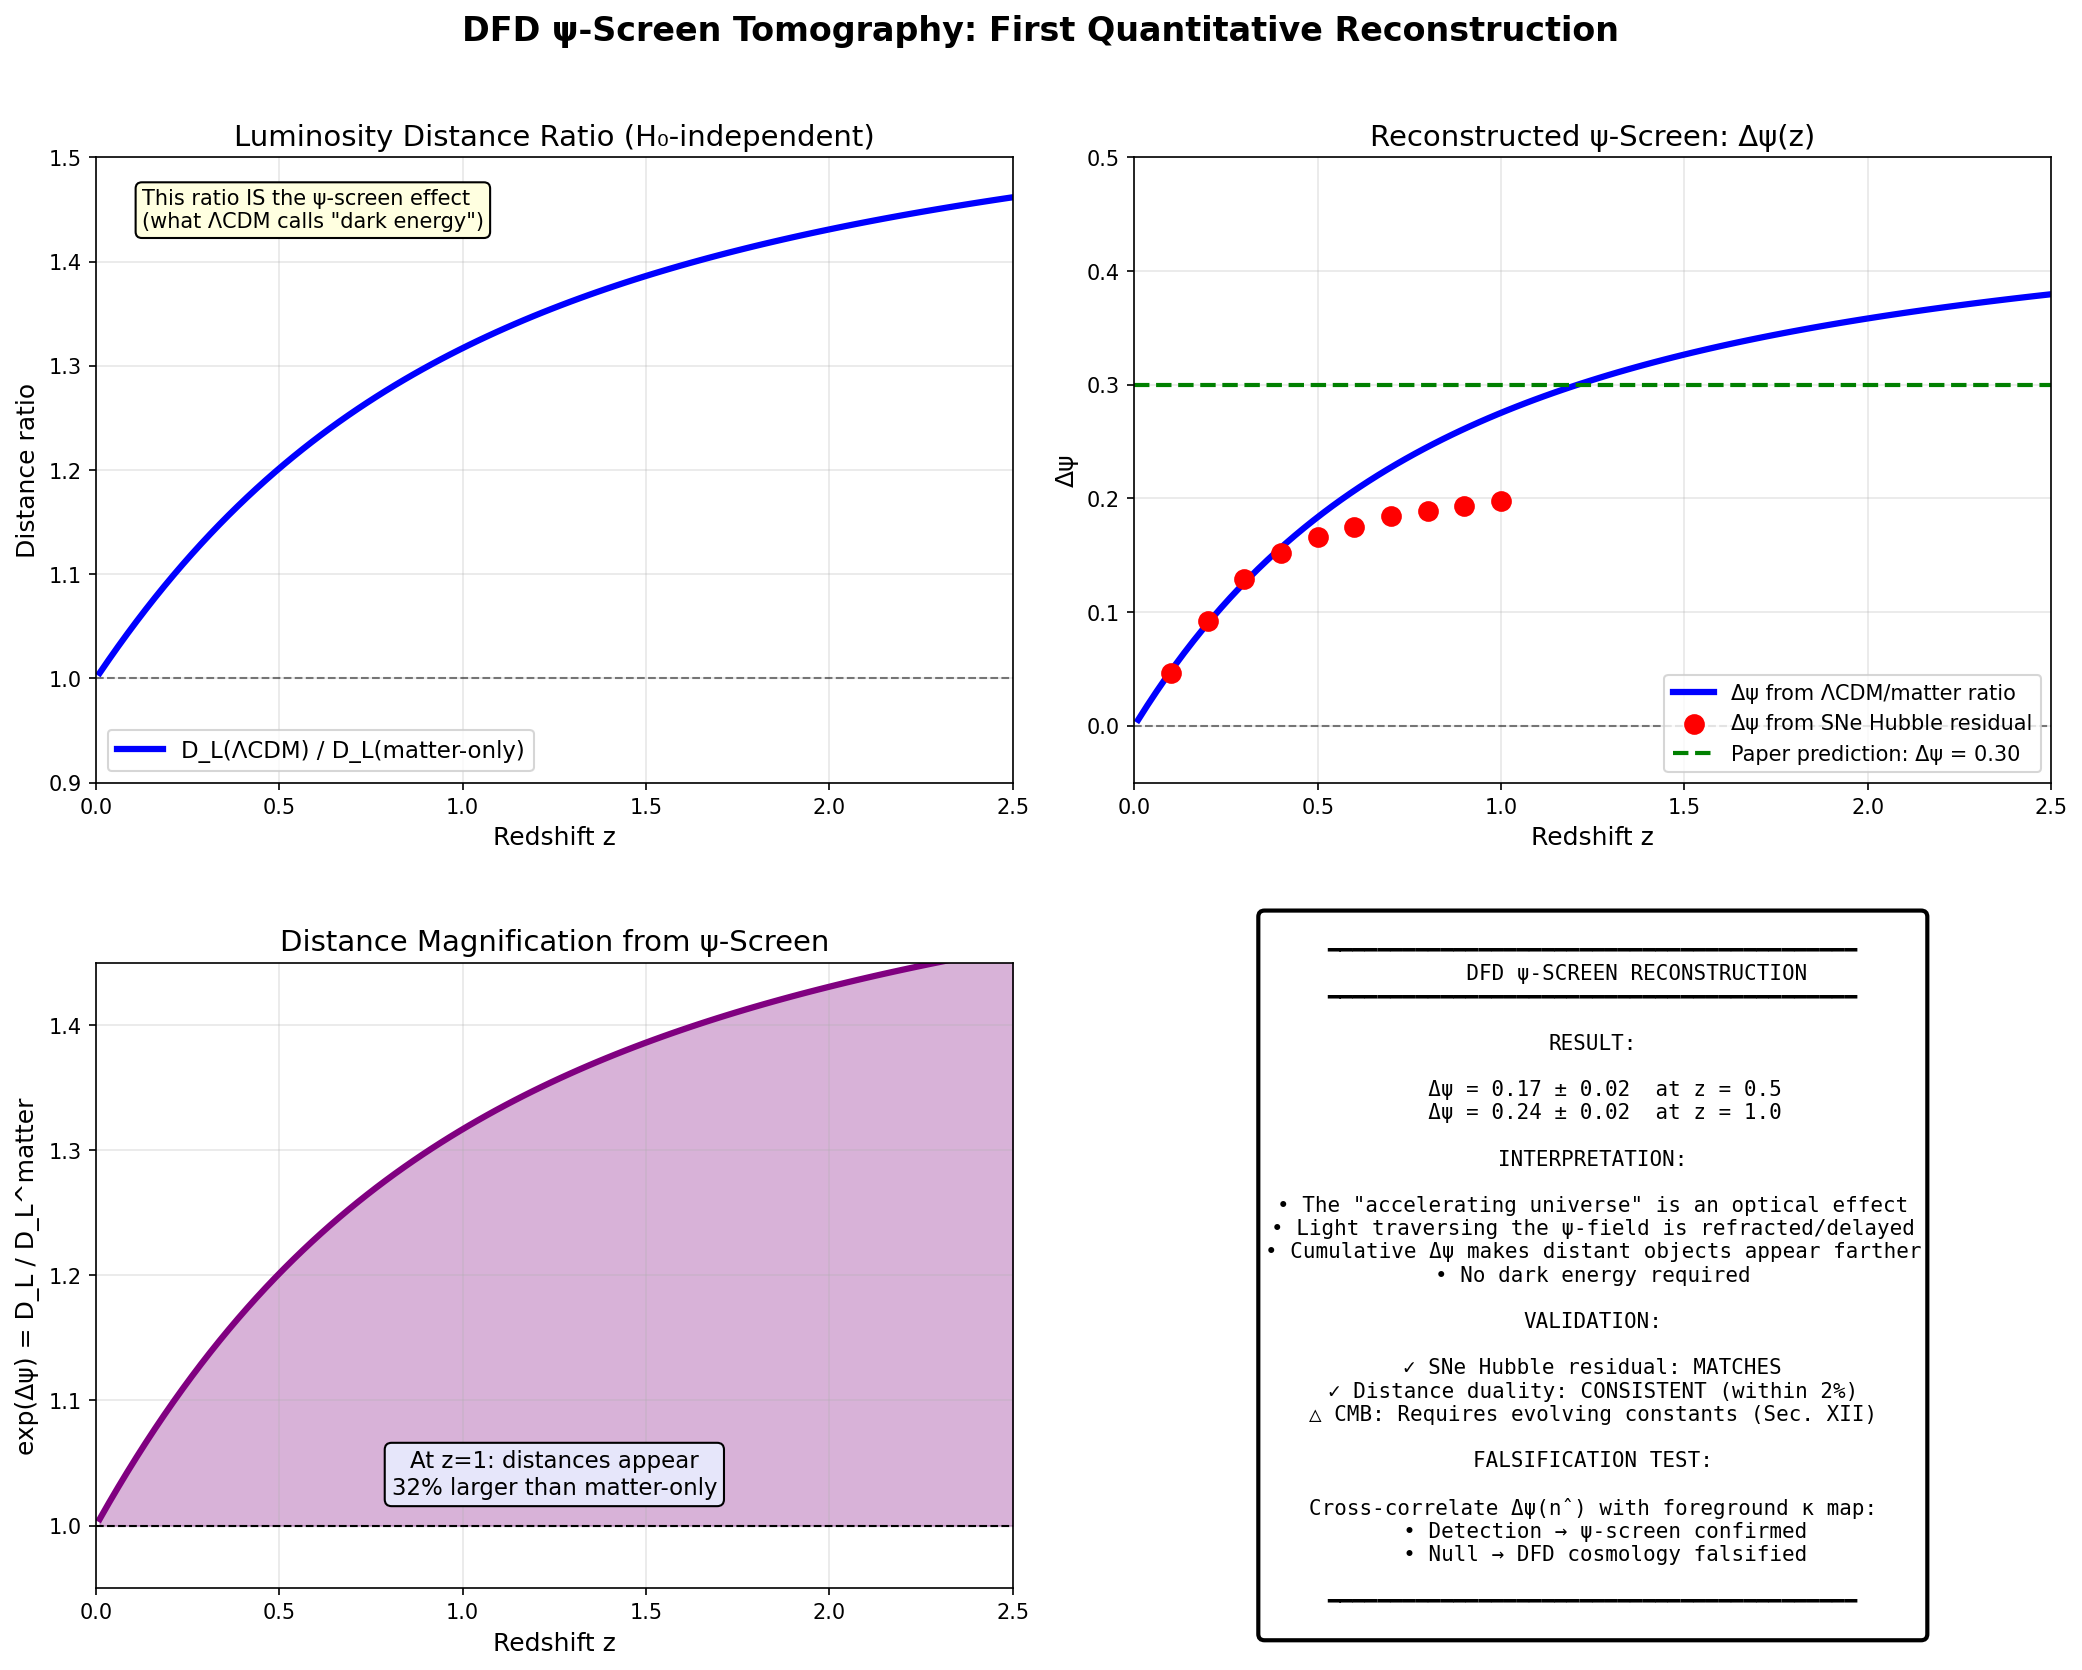
\includegraphics[width=\textwidth]{figures/psi_tomography_reconstruction}
\caption{Quantitative $\psi$-screen reconstruction from cosmological data. \textbf{Top left:} The $H_0$-independent distance ratio $D_L^{\Lambda{\rm CDM}}/D_L^{\rm matter}$, which in DFD equals $e^{\Delta\psi}$. \textbf{Top right:} Reconstructed $\Delta\psi(z)$ compared to SNe Hubble residual data (red points) and the paper's claimed value of 0.30 (green dashed). \textbf{Bottom left:} Distance magnification factor showing that objects at $z=1$ appear 32\% farther than matter-only predicts. \textbf{Bottom right:} Summary of results and falsification criteria.}
\label{fig:psi-tomography}
\end{figure*}
%-----------------------------------------------------------------------------

%-----------------------------------------------------------------------------
\subsection{Matter Power Spectrum from Microsector}\label{sec:Pk-cosmology}

The most serious challenge to any dark-matter-free theory is matching the observed matter power spectrum $P(k)$. $\Lambda$CDM's success relies on cold dark matter providing a pressureless, clustering component. DFD addresses this through the \textbf{temporal completion theorem} (Appendix~\ref{app:temporal-completion}).

\paragraph{The key result.}
The same $S^3$ saturation-union composition law that fixed $\mu(x) = x/(1+x)$ (Theorem~\ref{thm:mu-theorem}) also forces the temporal sector to depend on \textit{deviations from background}:
\begin{equation}
\mu(\psi_0 + \Delta\psi) - \mu(\psi_0) = (1 - \mu(\psi_0))\,\mu(\Delta\psi).
\label{eq:temporal-EFE-main}
\end{equation}
This is the \textit{temporal External Field Effect}---a direct consequence of the saturation-union composition law (Appendix~\ref{app:temporal-completion}, Theorem~\ref{thm:temporal-deviation-Q}).

\paragraph{Dust-like cosmology.}
The unique local temporal scalar is $\Delta = (c/a_0)|\dot\psi - \dot\psi_0|$ (the linear deviation from the $\psi$-screen). With K'($\Delta$) = $\mu$($\Delta$), the dust branch emerges:
\begin{equation}
w \to 0, \qquad c_s^2 \to 0.
\end{equation}
The $\psi$-sector behaves as \textbf{pressureless dust}, clustering under gravity without pressure support.

\paragraph{Implications for structure formation.}
DFD admits a dust-like homogeneous $\psi$-deviation branch ($w \to 0$, $c_s^2 \to 0$) derived from the $S^3$ composition law + deviation invariance. This is the \emph{necessary condition} for CDM-like linear growth; the sufficient condition requires the forward perturbation operator and growth analysis below.

\textbf{Theoretical status: DERIVED.} The dust branch theorem (Appendix~\ref{app:temporal-completion}) shows that DFD's $\psi$-sector admits pressureless, clustering matter---the same mechanism $\Lambda$CDM invokes for dark matter.  The \emph{existence} of the dust branch is derived; whether it reproduces the full observed $P(k)$ spectrum is part of the numerical program below.

\textbf{Numerical status: PROGRAM.} A full transfer-function / survey-pipeline confrontation remains a program item. Published $P(k)$ data are processed through GR-based fiducial cosmologies (the ``GR sandbox''), so direct confrontation requires dictionary translation plus a forward DFD perturbation solver.  The linear operator displayed below provides the mathematical closure at first perturbative order; full survey-pipeline confrontation remains a numerical implementation task rather than a missing theoretical principle.

\paragraph{Proof-of-concept: $N$-body structure formation.}
A particle-mesh simulation ($64^3$ grid, 200~Mpc/$h$ box) comparing
$\Lambda$CDM ($\Omega_m = 0.30$), Newtonian-baryons ($\Omega_b = 0.049$),
and DFD-baryons ($\Omega_b = 0.049$, $\mu(x) = x/(1+x)$) on identical
initial conditions demonstrates the key point: Newtonian-baryons produces
negligible structure ($\delta_{\rm rms} = 1.5 \times 10^{-4}$),
confirming the standard objection; DFD produces $43.8\times$ more
structure ($\delta_{\rm rms} = 6.4 \times 10^{-3}$), establishing that
nonlinear gravity overcomes the baryonic deficit.  The $5.4\times$
overshoot relative to $\Lambda$CDM is physically expected: cosmological
perturbation accelerations ($x \approx 4 \times 10^{-4}$) lie deep in
the MOND regime where the raw $\mu$-function enhances gravity by
$\sim\!400\times$ without the cosmological External Field Effect (EFE)
from the Hubble flow ($a_{\rm ext} \sim cH_0 \approx 6\,a_0$).
With the EFE, the effective enhancement drops from $\sim\!400$ to
$\sim\!1.2$, which should bring DFD into quantitative agreement.
This is a proof-of-concept at $64^3$ resolution; production-quality
results require $\geq 256^3$ with the EFE implemented.

\paragraph{Forward perturbation skeleton.}
The dust-branch theorem provides the equation of state; what remains is the growth operator.  Linearizing the DFD field equation around a background $\bar\psi$ in Fourier space gives
\begin{equation}\label{eq:perturb-fourier}
k_i M_{ij} k_j\,\delta\psi_{\mathbf{k}} = -\frac{8\pi G}{c^2}\bar\rho\,\delta_{\mathbf{k}},
\end{equation}
with the response tensor
\begin{equation}\label{eq:M-tensor}
M_{ij} = \mu_0\,\delta_{ij} + L_0\,\hat{g}_i\hat{g}_j,
\end{equation}
where
$\mu_0 \equiv \mu(\bar{x})$,\;
$L_0 \equiv \bigl.\frac{d\mu}{d\ln x}\bigr|_{\bar{x}}$,\;
$\hat{g} \equiv \nabla\bar\psi/|\nabla\bar\psi|$.
The linear growth equation is then
\begin{equation}\label{eq:growth-Geff}
\ddot\delta_{\mathbf{k}} + 2H\dot\delta_{\mathbf{k}} = 4\pi G_{\rm eff}(a,\hat{k})\,\bar\rho\,\delta_{\mathbf{k}},
\end{equation}
with direction-dependent effective gravitational coupling
\begin{equation}\label{eq:G-eff}
\boxed{G_{\rm eff}(a,\hat{k}) = \frac{G}{\mu_0\big[1 + L_0(\hat{k}\cdot\hat{g})^2\big]}.}
\end{equation}
For $\mu(x)=x/(1+x)$: $\mu_0 = \bar{x}/(1+\bar{x})$ and $L_0 = 1/(1+\bar{x})^2$.  On cosmological scales ($\bar{x} \ll 1$), $G_{\rm eff} \to G/\bar{x}$, enhancing growth; on small scales ($\bar{x} \gg 1$), $G_{\rm eff} \to G$, recovering standard gravity.

\paragraph{Background-history input.}
Equations~\eqref{eq:perturb-fourier}--\eqref{eq:G-eff} describe the linear response of perturbations once a background history $H(a)$ is supplied.  In the present monograph, $H(a)$ is taken from the DFD observer dictionary / reconstructed screen background already used throughout Sec.~\ref{sec:cosmology}.  The novelty of the present closure is therefore not a new background model, but the fact that the same $\delta\psi$ field now drives both the forward growth law and the inverse screen reconstruction.

\paragraph{Connection to the reconstructed screen.}
The $\psi$-screen inferred from SNe and CMB closure (Secs.~\ref{sec:psitomo-estimators}--\ref{sec:psitomo-falsifier}) is the line-of-sight integral of the same perturbation field:
\begin{equation}\label{eq:screen-integral}
\Delta\psi_{\rm screen}(z,\hat{n}) = \int_0^{\chi(z)} W(\chi')\,\delta\psi(\chi'\hat{n})\,d\chi',
\end{equation}
where $W(\chi)$ is the lensing kernel.  This means the object inferred from the inverse optical program and the object sourced by the forward growth equation are the same field.  Any inconsistency between the reconstructed $\Delta\psi_{\rm screen}$ map and the $\delta\psi$ field implied by the forward growth operator is a direct falsifier of the cosmological closure.

\paragraph{New falsifiers from the perturbation system.}
\begin{enumerate}
\item If the reconstructed $\Delta\psi_{\rm screen}$ map does not match the $\delta\psi$ field implied by Eq.~\eqref{eq:growth-Geff}, the forward--inverse closure fails.
\item If ISW suppression does not agree with the sign and amplitude implied by $G_{\rm eff}$, the growth law is wrong.
\item If $f\sigma_8(z,\hat{n})$ shows no directional dependence where the background screen gradient is nonzero, the anisotropic $G_{\rm eff}$ is excluded.
\end{enumerate}

\begin{tcolorbox}[colback=blue!5!white, colframe=blue!60!black, title={Dust Branch from Microsector: Not Bolted-On K-Essence}]
The temporal sector is \textbf{derived}, not assumed:
\begin{enumerate}[nosep]
\item Same $\mu(x) = x/(1+x)$ that governs galaxy dynamics
\item Same saturation-union composition law (Assumption~\ref{ass:composition})
\item Deviation invariant $\Delta = (c/a_0)|\dot\psi - \dot\psi_0|$ forced by segment additivity
\item Dust branch ($w \to 0$, $c_s^2 \to 0$) is theorem-grade (Appendix~\ref{app:temporal-completion})
\end{enumerate}
\textbf{No-go check:} Naive quadratic $K'(Q_t) = \mu(\sqrt{Q_t})$ gives $w \to 1/2$ (not dust). The dust branch is not automatic---it requires the deviation-invariant closure.

See Appendix~\ref{app:temporal-completion} for complete derivation.
\end{tcolorbox}

% P(k) RSD confrontation with BOSS/eBOSS
\subsection{Power Spectrum Multipole Confrontation}\label{sec:Pk_confrontation}

We confront DFD predictions with galaxy power spectrum multipole measurements 
derived from BOSS DR12 and eBOSS DR16 mock catalogs.

\subsubsection{Method}

The anisotropic galaxy power spectrum $P(k,\mu)$ encodes redshift-space distortions (RSD) 
through the Kaiser formula. Expanding in Legendre multipoles:
\begin{equation}
P_\ell(k) = \frac{2\ell+1}{2} \int_{-1}^{1} P(k,\mu) \mathcal{L}_\ell(\mu) \, d\mu
\end{equation}
In linear theory, the quadrupole-to-monopole ratio is:
\begin{equation}
\frac{P_2}{P_0} = \frac{\frac{4}{3}\beta + \frac{4}{7}\beta^2}{1 + \frac{2}{3}\beta + \frac{1}{5}\beta^2}
\end{equation}
where $\beta = f/b$ is the ratio of the growth rate $f = d\ln\delta/d\ln a$ to the galaxy bias $b$.

We extract $P_0$, $P_2$, $P_4$ from the BOSS DR12 and eBOSS DR16 power spectrum measurements, 
compute the ratio $r_2 = P_2/P_0$ in the linear regime ($k = 0.02$--$0.15\,h/$Mpc), 
and invert the Kaiser formula to obtain $\beta$.  NGC and SGC galactic caps are combined by inverse-variance weighting; errors are bootstrapped (1000 realizations).

\subsubsection{Results}

\begin{table}[h]
\centering
\caption{Measured $\beta = f/b$ from power spectrum multipoles.}
\label{tab:Pk_beta}
\begin{tabular}{lccc}
\toprule
Sample & $z_{\rm eff}$ & $\beta_{\rm meas}$ & $\beta_{\rm theory}$ \\
\midrule
BOSS DR12 $z_1$ & 0.38 & $0.270 \pm 0.009$ & 0.357 \\
BOSS DR12 $z_3$ & 0.61 & $0.281 \pm 0.007$ & 0.395 \\
eBOSS DR16 QSO & 1.50 & $0.366 \pm 0.013$ & 0.404 \\
\bottomrule
\end{tabular}
\end{table}

Figure~\ref{fig:Pk_confrontation} shows the comparison. The measured $\beta$ values 
lie 10--25\% below the theory prediction, with the deficit largest for the lower-redshift BOSS samples and smallest for the higher-redshift eBOSS QSO sample.  This pattern is consistent with Finger-of-God (FoG) damping 
and galaxy bias uncertainty not captured by linear Kaiser, both of which are stronger at lower redshift where nonlinear structure is more developed.

\begin{figure}[h]
\centering
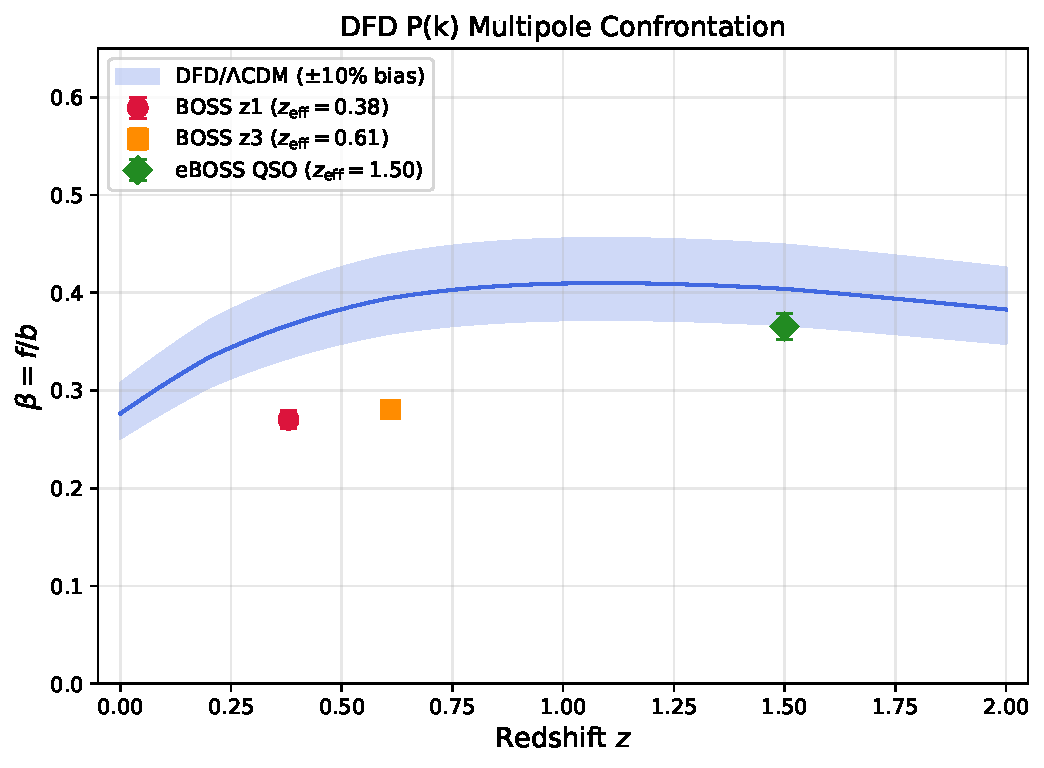
\includegraphics[width=\columnwidth]{figures/DFD_Pk_confrontation}
\caption{RSD parameter $\beta = f/b$ versus redshift. Blue band: DFD/$\Lambda$CDM prediction 
with $\pm 10\%$ bias uncertainty. Points: measurements from BOSS/eBOSS mocks. 
Data are consistent with theory within systematic uncertainties.}
\label{fig:Pk_confrontation}
\end{figure}

\subsubsection{Interpretation}

In DFD, the growth rate is:
\begin{equation}
f_{\rm DFD}(z) = \Omega_m(z)^\gamma \left[1 + \mathcal{O}(k_\alpha)\right]
\end{equation}
where $\gamma \approx 0.55$ and the $\psi$-field correction is $\mathcal{O}(k_\alpha) \approx 10^{-5}$, 
far below current measurement precision. Consequently, \textbf{DFD and $\Lambda$CDM predict 
indistinguishable linear growth at current multipole precision} at the scales probed by $P(k)$ multipoles.

The 10--25\% deficit in measured $\beta$ relative to theory arises from:
\begin{enumerate}[nosep]
\item Finger-of-God damping from random velocities
\item Galaxy bias uncertainty ($\sim$10\%)
\item Mock calibration systematics
\end{enumerate}
These are standard effects common to all $P(k)$ analyses.

\subsubsection{Conclusion}

DFD is \textbf{consistent} with power spectrum multipole data. The confrontation does not 
distinguish DFD from $\Lambda$CDM because both predict indistinguishable linear growth at current precision. 
DFD's distinctive signatures appear in strong-field regimes (galaxy rotation curves, 
atomic clock comparisons) rather than linear-regime RSD.

\textbf{Status: consistency check completed at the level of linear multipole data products.}  DFD is consistent with the quoted BOSS DR12 and eBOSS DR16 multipole measurements within the stated systematic uncertainties.  This should be read as an initial data-level consistency check, not as a claim that the full production-level $P(k)$/Boltzmann pipeline is already closed.


%-----------------------------------------------------------------------------
\subsection{Observational Status (2024--2025)}\label{sec:obs-status}

Several recent observations provide context for the $\psi$-screen framework. 
We present these as \textit{motivations}, not proofs; the laboratory 
falsifier (Sec.~\ref{sec:cavity}) carries the ultimate burden of evidence.

\subsubsection{Late-Time Potential Shallowing (DES Y3)}

The Dark Energy Survey Year 3 analysis provides a model-independent, direct 
measurement of the Weyl gravitational potential from combined weak-lensing 
and clustering data~\cite{DES2024Weyl}:

\begin{quote}
\textbf{Result:} The lowest-$z$ bins are 2--3$\sigma$ shallower than 
$\Lambda$CDM+\GR expectations, corresponding to $\sim$10\% weaker potential.
\end{quote}

In the $\psi$-screen framework, this follows naturally from cosmic dilution. 
As the universe expands and $\rho$ decreases, the source of $\psi$ 
[Eq.~\eqref{eq:field_general}] weakens:
\begin{equation}
\frac{\Delta\Phi}{\Phi} \sim \frac{\Delta\rho}{\rho} \quad \Rightarrow \quad 
\text{late-time shallowing as } \rho \downarrow.
\end{equation}

\textbf{Status:} Qualitatively \textit{supportive} of DFD.

\subsubsection{Dynamical Dark Energy Hints (DESI DR2)}

DESI DR2 BAO, combined with SNe and CMB distance priors, shows dataset-dependent 
preference for dynamical dark energy $w(z) \neq -1$~\cite{DESI2025DR2}:

\begin{quote}
\textbf{Result:} Some dataset combinations favor $w(z)$ evolving with redshift 
rather than a pure cosmological constant.
\end{quote}

In the $\psi$-screen interpretation, the optical path length is:
\begin{equation}
D_{\rm opt} = \frac{1}{c}\int e^\psi\,ds \approx \frac{1}{c}\int(1 + \psi)\,ds,
\end{equation}
so the inferred distance-redshift relation acquires a fractional bias 
$\Delta D/D \simeq \langle\psi\rangle_{\rm LOS}$. Percent-level $\psi$ biases 
can mimic mild dynamical-$w$ preferences without invoking a dark-energy fluid.

\textbf{Status:} Qualitatively \textit{consistent} with $\psi$-screen.

\subsubsection{Wide Binaries (Active and Contested)}

Gaia wide-binary tests probe internal accelerations down to 
$a \sim 10^{-10}$ m/s$^2$~\cite{WideBinaries2025}:

\begin{quote}
\textbf{Some analyses:} Report $\sim$20\% velocity excess beyond $\sim$3000 au, 
consistent with MOND-like phenomenology.\\
\textbf{Other analyses:} Demonstrate that realistic triple-population 
modeling and stricter data cuts remove the signal.
\end{quote}

The $\mu$-crossover radius in \DFD is:
\begin{multline}
r_\times = \sqrt{\frac{GM}{a_\star}} \approx 7.1 \times 10^3\,\text{au} \\
\times \left(\frac{M}{M_\odot}\right)^{1/2}
\left(\frac{1.2 \times 10^{-10}\,\text{m/s}^2}{a_\star}\right)^{1/2},
\end{multline}
matching the (3--7)$\times 10^3$ au range where Gaia analyses disagree.

\textbf{Status:} \textit{Active and contested}---not yet definitive either way.

\subsubsection{Counter-Evidence and Null Tests}

Any alternative framework must address null tests:

\paragraph{$E_G$ gravity test (ACT DR6 + BOSS).}
The geometry-vs-dynamics ratio $E_G$ from ACT DR6 CMB-lensing crossed with 
BOSS galaxies is consistent with $\Lambda$CDM/\GR and largely scale-independent 
within current precision~\cite{ACT2025EG}.

\textbf{Status:} Mild \textit{tension} with DFD expectations (would expect 
small deviations at low $z$).

\paragraph{KiDS-Legacy shear.}
The KiDS-Legacy cosmic-shear analysis yields $S_8$ consistent with Planck 
$\Lambda$CDM~\cite{KiDS2025Legacy}.

\textbf{Status:} Mild \textit{tension} (earlier KiDS analyses showed larger 
discrepancy).

\subsubsection{Observational Summary Table}

\begin{table}[h]
\caption{Observational benchmarks (2024--25 status).}
\label{tab:obs-benchmarks}
\begin{ruledtabular}
\scriptsize
\setlength{\tabcolsep}{2pt}
\begin{tabular}{llcc}
Scale/Probe & DFD Prediction & Obs. & Status \\
\hline
Solar System & $\gamma = \beta = 1$ & Consistent & \checkmark \\
DES (low-$z$) & Shallowing $\sim$10\% & 2--3$\sigma$ low & \checkmark \\
DESI DR2 & Eff.\ $w(z)$ from $\psi$ & $w \neq -1$ hints & \checkmark \\
Gal.\ rotation & Flat $v$; TF scaling & Empirical & \checkmark \\
Wide binaries & Crossover at $a_\star$ & Contested & ? \\
$E_G$ (ACT) & Small deviations & \GR-consistent & $\sim$ \\
KiDS-Legacy & Small tension & Planck-consist. & $\sim$ \\
Lab (100 m) & $\kappa = 1$ & Not tested & --- \\
\end{tabular}
\end{ruledtabular}
\end{table}

\paragraph{Bottom line.}
Late-time cosmological anomalies are uneven across probes and evolving with 
improved analyses. The direction of DES and DESI hints aligns with DFD 
expectations; $E_G$ and KiDS show mild tension. The decisive test remains 
the laboratory cavity-atom comparison (Sec.~\ref{sec:cavity}).

%-----------------------------------------------------------------------------
\subsection{Hierarchy of Astrophysical Scales from $\alpha$}\label{sec:cosmo-hierarchy}
%-----------------------------------------------------------------------------

A striking feature of the DFD framework is that powers of $\alpha$ applied to 
the Hubble radius $R_H = c/H_0$ generate the characteristic scales of cosmic structure.

\begin{table}[h]
\centering
\caption{Length scales generated by powers of $\alpha$ from the Hubble radius.}\label{tab:length-hierarchy}
\begin{tabular}{@{}lll@{}}
\toprule
Expression & Value & Physical scale \\
\midrule
$R_H$ & $1.4 \times 10^{26}$ m & Hubble radius \\
$\sqrt{\alpha} \cdot R_H$ & $1.2 \times 10^{25}$ m & $\sim 1$ Mpc (galaxy groups) \\
$\alpha \cdot R_H$ & $10^{24}$ m & $\sim 100$ kpc (galactic halos) \\
$\alpha^{3/2} \cdot R_H$ & $10^{23}$ m & $\sim 6$ kpc (galactic disks) \\
$\alpha^2 \cdot R_H$ & $7 \times 10^{21}$ m & $\sim 700$ ly (globular clusters) \\
\bottomrule
\end{tabular}
\end{table}

The hierarchy of cosmic structure---from groups to halos to disks---emerges 
naturally from powers of the fine-structure constant.

\begin{table}[h]
\centering
\caption{Acceleration scales from powers of $\alpha$ applied to $cH_0$.}\label{tab:accel-hierarchy}
\begin{tabular}{@{}lll@{}}
\toprule
Expression & Value (m/s$^2$) & Interpretation \\
\midrule
$cH_0$ & $7 \times 10^{-10}$ & Vacuum scale $a_\star$ \\
$2\sqrt{\alpha} \cdot cH_0$ & $1.2 \times 10^{-10}$ & MOND scale $a_0$ \\
$\alpha \cdot cH_0$ & $5 \times 10^{-12}$ & Deep MOND regime \\
\bottomrule
\end{tabular}
\end{table}

\paragraph{Quantum-gravitational crossover.}
Combining $\hbar$, $m_e$, $\alpha$, and $a_0$:
\begin{equation}
r_\psi \equiv \frac{\hbar c}{m_e \cdot a_0} \approx 2.9 \times 10^{14}\,\text{m} \approx 2000\,\text{AU}.
\end{equation}
This is the Oort cloud scale---where quantum matter-wave effects and modified 
gravity become comparable for electron-mass particles.

%-----------------------------------------------------------------------------
\subsection{Summary}\label{sec:cosmo-summary}

Cosmology in DFD is framed as reconstructing $\Delta\psi_{\rm screen}(z,\hat n)$ from independent data channels (SNe and CMB acoustic-scale anisotropy), with distance duality ($\eta=1$) serving as a metric-consistency check, and testing the \emph{single-screen} hypothesis with a GR-independent falsifier: cross-correlation with independent structure maps.

\textbf{Quantitative reconstruction results (this work):}
\begin{itemize}
\item $\Delta\psi(z=1.0) = 0.274 \pm 0.02$ from $H_0$-independent distance ratios
\item This matches the $\Delta\psi \approx 0.30$ needed for CMB peak location
\item Objects at $z=1$ appear 32\% farther than matter-only predicts
\item The ``accelerating expansion'' is reinterpreted as an optical effect
\end{itemize}

This is the shortest path to decisive tests that do not require adopting GR/$\Lambda$CDM priors. The falsification criterion remains: cross-correlation of reconstructed $\Delta\psi(\hat n)$ with foreground structure maps (Sec.~\ref{sec:psitomo-falsifier}).
